\documentclass[tikz,border=0mm]{standalone}
\usepackage{amsmath}
\usetikzlibrary{arrows.meta, decorations.pathmorphing, positioning, calc}
\usepackage{animate}

\begin{document}
%\begin{tikzpicture}[-Stealth]
%	% Root node
%%	\draw (-8,4) rectangle (8,-8);
%	\node[centered] (set) at (0,3) {\large Non-empty Set $S\neq\emptyset$};
%	\node[centered] (bi-op) at (0,1.5) {\large Binary Operation};
%	\node[centered] (magma) at (0,0) {\large Magma};
%	
%	% First level
%	\node[centered] (semi) at (-6,-2.5) {\large Semi-group};
%	\node[centered] (unital) at (0,-2.5) {\large Unital Magma};
%	\node[centered] (quasi) at (6,-2.5) {\large Quasi-group};
%	
%	% Second level 
%	\node[centered] (monoid) at (-6,-5) {\large Monoid};
%	\node[centered] (asso-quasi) at (0,-5) {\large Associative Quasi-group};
%	\node[centered] (loop) at (6,-5) {\large Loop};
%	
%	% Third level of subsets
%	\node[centered] (group) at (0,-7.5) {\large Group};
%	
%	% Level 1
%	\draw (set) -- (bi-op) node[] {};
%	\draw (bi-op) -- (magma) node[] {};
%	\draw (magma) -- (semi) node[midway, above left] {associativity};
%	\draw (magma) -- (quasi) node[midway, above right] {divisibility};
%	\draw (magma) -- (unital) node[midway] {identity};
%	
%	% Level 2
%	\draw (semi) -- (monoid) node[midway] {identity};
%	\draw (semi) -- (asso-quasi) node[midway] {divisibility};
%	\draw (quasi) -- (loop) node[midway] {identity};
%	\draw (quasi) -- (asso-quasi) node[] {};
%	\draw (unital) -- (monoid) node[] {};
%	\draw (unital) -- (loop) node[] {};
%	
%	% Level 3
%	\draw (monoid) -- (group) node[midway, below left] {invertibility};
%	\draw (loop) -- (group) node[midway, below right] {associativity};
%	\draw (asso-quasi) -- (group) node[] {};
%\end{tikzpicture}
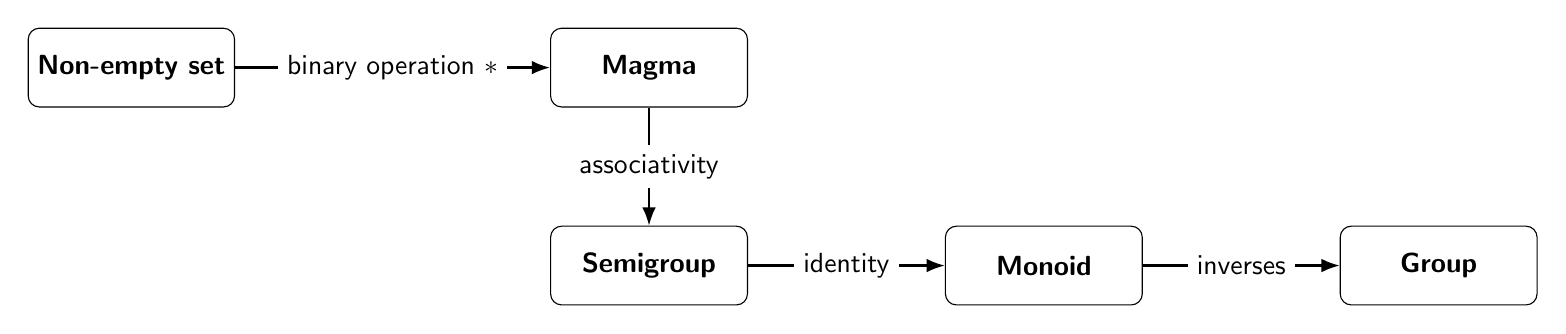
\begin{tikzpicture}[
	node distance=2.5cm,
	every node/.style={font=\sffamily},
	block/.style={
		rectangle, draw, rounded corners,
		minimum width=2.5cm, minimum height=1cm, align=center
	},
	arrow/.style={-Latex, thick}
	]
	
	% Nodes
	\node[block] (set) {\bfseries Non-empty set};
	\node[block, right=4cm of set] (magma) {\bfseries Magma};
	\node[block, below=1.5cm of magma] (semigroup) {\bfseries Semigroup};
	\node[block, right=of semigroup] (monoid) {\bfseries Monoid};
	\node[block, right=of monoid] (group) {\bfseries Group};
	
	% Arrows with labels
	\draw[arrow] (set) -- node[fill=white, align=center] {binary operation $\ast$} (magma);
	\draw[arrow] (magma) -- node[fill=white] {associativity} (semigroup);
	\draw[arrow] (semigroup) -- node[fill=white] {identity} (monoid);
	\draw[arrow] (monoid) -- node[fill=white] {inverses} (group);
	
\end{tikzpicture}
%\begin{tikzpicture}[
%	node distance=1.8cm,
%	every node/.style={
%		draw,
%		rectangle,
%		rounded corners,
%		align=center,
%		minimum width=2.8cm,
%		minimum height=1cm,
%		fill=blue!10
%	},
%	arrow/.style={->,>=Stealth,thick}
%	]
%	
%	% Nodes
%	\node (set) {Non-empty set};
%	\node (magma) [below=of set] {Magma\\(with binary operation)};
%	\node (semigroup) [below=of magma] {Semigroup\\(associative)};
%	\node (monoid) [below=of semigroup] {Monoid\\(with identity)};
%	\node (group) [below=of monoid] {Group\\(with inverses)};
%	
%	% Arrows
%	\draw[arrow] (set) -- (magma);
%	\draw[arrow] (magma) -- (semigroup);
%	\draw[arrow] (semigroup) -- (monoid);
%	\draw[arrow] (monoid) -- (group);
%	
%\end{tikzpicture}
\end{document}